
\chapter{Bisimulazione}


\section{Definizione di bisimulazione}

Siano $\mu=(S,\, R,\, V)$ e $\mu'=(S',\, R',\, V')$ due modelli
e siano $s\in S$, e $t\in S'$ due stati

Si dice che le coppie $(\mu,\, s)$ e $(\mu',\, s)$ sono in bisimulazione
tra loro, ossia:

$(\mu,\, s)\leftrightarroweq(\mu',\, s)$

Se esiste una relazione $E:S\times S$ tale che
\begin{enumerate}
\item $(s,\, t)\in E$
\item se $(x,\, y)\in E$ allora:\\
a)$\forall P\in\phi\, x\in V(P)\iff y\in V'(P)$\\
b1)$(x,\, z)\in R\implies\exists u\in S'\,:\,(y,\, u)\in R'\,\wedge\,(z,\, u)\in E$\\
b2)$(y,\, u)\in R'\implies\exists z\in S\,:\,(x,\, z)\in R\,\wedge\,(z,\, u)\in E$
\end{enumerate}
Due frame sono in bisimulazione se soddisfano le condizioni 1, b1
e b2.


\subsection{Teorema}

se $(\mu,\, s)\leftrightarroweq(\mu',\, s)$

allora: 

$\forall\varphi\in\phi\,\veraw{\mu}s{\varphi}\iff\veraw{\mu'}t{\varphi}$


\section{Esempi di bisimulazione}


\subsection{Alberi binari e Retta}

Consideriamo il frame rappresentante la lettera dei numeri naturali:

$N=(\mathbb{N},\, successivo)$

E il farme che rappresenta un albero binario a dimensione infinita:

$B=(w=\{0,\,1\}*,\,\rho)$

Supponiamo che V su B sia: 

$V(P)=\{w\in\{0,\,1\}*\,:\,|w|=2n\}$

Allora esiste una unica valutazione V' su N tale che $(B,\, V,\,0)\leftrightarroweq(N,\, V',\,\epsilon)$,
ed è:

$V'(P)=\mathbb{P}$ (l'insieme dei numeri pari)

Dimostriamolo per induzione:

$(n,\, w)\in E\iff|w|=n$

il caso base si dimostra banalmente:

$|\epsilon|=0$

$(\epsilon,\,0)\in E$

per definizione. Per il passo induttivo abbiamo:

$|w|=n$

$(w,\, n)\in E$

sia w per ipotesi tale che $|w|=n+1$

allora:

$w=ua$, $|u|=n$, $a\in\{0,\,1\}$

per la condizione 1 di bisimulazione:

$(u,\, w)\in\rho$ e $(u,\, n)\in E$

per la condizione b1 invece:

$\exists m\in\mathbb{N}\,:\, m=n+1\wedge(w,\, n+1)\in E$

e quindi si deduce facilmente che:

$|w|=|ua|=n+1$

e quindi la valutazione non può che essere la sola V', perchè è qualla
che si ricava imponendo la condizione di bisimulazione, e che rispetta
anche la condizione 2.

\begin{center} 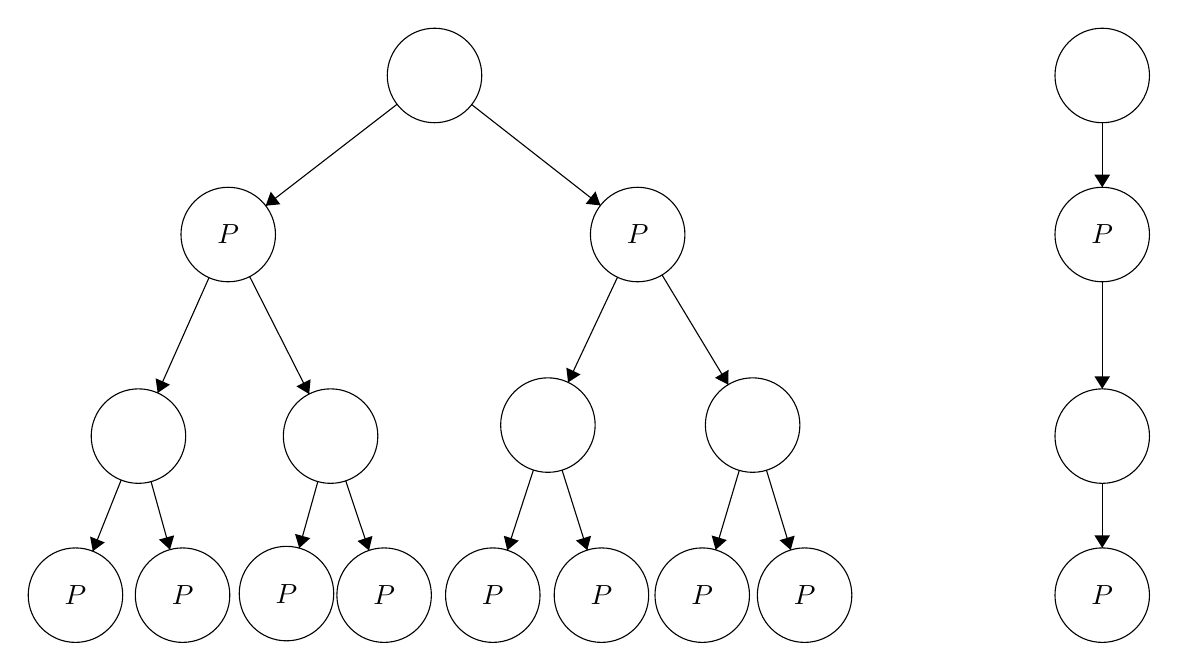
\begin{tikzpicture}[scale=0.2] \tikzstyle{every node}+=[inner sep=0pt] \draw [black] (26.2,-6.3) circle (3); \draw [black] (13.1,-16.4) circle (3); \draw (13.1,-16.4) node {$P$}; \draw [black] (39.1,-16.4) circle (3); \draw (39.1,-16.4) node {$P$}; \draw [black] (7.4,-29.2) circle (3); \draw [black] (19.6,-29.2) circle (3); \draw [black] (33.4,-28.5) circle (3); \draw [black] (46.4,-28.5) circle (3); \draw [black] (3.4,-39.3) circle (3); \draw (3.4,-39.3) node {$P$}; \draw [black] (10.2,-39.3) circle (3); \draw (10.2,-39.3) node {$P$}; \draw [black] (16.8,-39.2) circle (3); \draw (16.8,-39.2) node {$P$}; \draw [black] (23,-39.3) circle (3); \draw (23,-39.3) node {$P$}; \draw [black] (29.9,-39.3) circle (3); \draw (29.9,-39.3) node {$P$}; \draw [black] (36.8,-39.3) circle (3); \draw (36.8,-39.3) node {$P$}; \draw [black] (43.2,-39.3) circle (3); \draw (43.2,-39.3) node {$P$}; \draw [black] (49.7,-39.3) circle (3); \draw (49.7,-39.3) node {$P$}; \draw [black] (68.6,-6.3) circle (3); \draw [black] (68.6,-16.4) circle (3); \draw (68.6,-16.4) node {$P$}; \draw [black] (68.6,-29.2) circle (3); \draw [black] (68.6,-39.3) circle (3); \draw (68.6,-39.3) node {$P$}; \draw [black] (23.82,-8.13) -- (15.48,-14.57); \fill [black] (15.48,-14.57) -- (16.41,-14.48) -- (15.8,-13.68); \draw [black] (28.56,-8.15) -- (36.74,-14.55); \fill [black] (36.74,-14.55) -- (36.42,-13.66) -- (35.8,-14.45); \draw [black] (11.88,-19.14) -- (8.62,-26.46); \fill [black] (8.62,-26.46) -- (9.4,-25.93) -- (8.49,-25.53); \draw [black] (14.46,-19.07) -- (18.24,-26.53); \fill [black] (18.24,-26.53) -- (18.33,-25.59) -- (17.43,-26.04); \draw [black] (37.82,-19.11) -- (34.68,-25.79); \fill [black] (34.68,-25.79) -- (35.47,-25.28) -- (34.57,-24.85); \draw [black] (40.65,-18.97) -- (44.85,-25.93); \fill [black] (44.85,-25.93) -- (44.87,-24.99) -- (44.01,-25.5); \draw [black] (6.3,-31.99) -- (4.5,-36.51); \fill [black] (4.5,-36.51) -- (5.26,-35.95) -- (4.33,-35.58); \draw [black] (8.2,-32.09) -- (9.4,-36.41); \fill [black] (9.4,-36.41) -- (9.67,-35.5) -- (8.7,-35.77); \draw [black] (18.79,-32.09) -- (17.61,-36.31); \fill [black] (17.61,-36.31) -- (18.31,-35.68) -- (17.34,-35.41); \draw [black] (20.56,-32.04) -- (22.04,-36.46); \fill [black] (22.04,-36.46) -- (22.26,-35.54) -- (21.31,-35.86); \draw [black] (32.48,-31.35) -- (30.82,-36.45); \fill [black] (30.82,-36.45) -- (31.55,-35.84) -- (30.6,-35.53); \draw [black] (34.3,-31.36) -- (35.9,-36.44); \fill [black] (35.9,-36.44) -- (36.14,-35.53) -- (35.18,-35.83); \draw [black] (45.55,-31.38) -- (44.05,-36.42); \fill [black] (44.05,-36.42) -- (44.76,-35.8) -- (43.8,-35.51); \draw [black] (47.28,-31.37) -- (48.82,-36.43); \fill [black] (48.82,-36.43) -- (49.07,-35.52) -- (48.11,-35.81); \draw [black] (68.6,-9.3) -- (68.6,-13.4); \fill [black] (68.6,-13.4) -- (69.1,-12.6) -- (68.1,-12.6); \draw [black] (68.6,-19.4) -- (68.6,-26.2); \fill [black] (68.6,-26.2) -- (69.1,-25.4) -- (68.1,-25.4); \draw [black] (68.6,-32.2) -- (68.6,-36.3); \fill [black] (68.6,-36.3) -- (69.1,-35.5) -- (68.1,-35.5); \end{tikzpicture} \end{center}


\subsection{Alberi binari e frame finito}

Supponiamo di prendere su un frame binario B la seguante funzione
di valutazione:

$V(P)=\{0w\,|\, w\in\{0,1\}*\}$

$V(Q)=\{1w\,|\, w\in\{0,1\}*\}$

In questo frame Q è vera su tutto il sottoalbero destro, mentre P
sul sottoalbero sinistro.

è evidente che non può esistere alcuna V' su N tale che $(B,\, V,\,0)\leftrightarroweq(N,\, V',\,\epsilon)$,
erchè dovrebbero esistere due insiemi di stati non in relazione tra
loro per cui in uno valga P e nell'altro Q. Ma questo non è possibile,
poichè il frame N è una retta di elementi connessi a uno a uno. Tuttavia
esiste un frame molto più semplice e finito che bisimula l'albero,
di soli 3 stati, uno per lo stato $\epsilon$, uno per lo stato in
qui vale P, e uno per lo stato in cui vale Q. Si può vedere come l'automa
che riconosce se la stringa è ``etichettatta'' P o Q.

\begin{center} \begin{tikzpicture}[scale=0.2] \tikzstyle{every node}+=[inner sep=0pt] \draw [black] (39.2,-9.7) circle (3); \draw [black] (25.5,-25.3) circle (3); \draw (25.5,-25.3) node {$P$}; \draw [black] (53,-25.3) circle (3); \draw (53,-25.3) node {$Q$}; \draw [black] (37.22,-11.95) -- (27.48,-23.05); \fill [black] (27.48,-23.05) -- (28.38,-22.77) -- (27.63,-22.11); \draw [black] (24.182,-27.982) arc (1.56859:-286.43141:2.25); \fill [black] (22.57,-25.89) -- (21.76,-25.41) -- (21.78,-26.41); \draw [black] (55.83,-26.26) arc (99:-189:2.25); \fill [black] (53.96,-28.13) -- (53.59,-29) -- (54.58,-28.84); \draw [black] (41.19,-11.95) -- (51.01,-23.05); \fill [black] (51.01,-23.05) -- (50.86,-22.12) -- (50.11,-22.79); \end{tikzpicture} \end{center} 


\subsection{Infiniti cammini vs Cammino infinito}

Consideriamo due frame, il primo tale che da un nodo $\alpha$ partono
infiniti percorsi, e l'altro che ha un solo percorso di lunghezza
infinita. 

\begin{center} 
\begin{tikzpicture}[scale=0.2] 
\tikzstyle{every node}+=[inner sep=0pt] 
\draw [black] (36,-8.8) circle (3); 
\draw (36,-8.8) node {$\alpha$}; 
\draw [black] (27.8,-21.8) circle (3); 
\draw [black] (22.6,-31.4) circle (3); 
\draw [black] (43.5,-21.1) circle (3); 
\draw [black] (50.4,-31.4) circle (3); 
\draw [black] (57.6,-41.3) circle (3); 
\draw (58.9,-15.2) node {$...$}; 
\draw [black] (12.1,-19.2) circle (3); 
\draw [black] (33.25,-10) -- (14.85,-18); 
\fill [black] (14.85,-18) -- (15.78,-18.14) -- (15.38,-17.23); 
\draw [black] (34.4,-11.34) -- (29.4,-19.26); 
\fill [black] (29.4,-19.26) -- (30.25,-18.85) -- (29.4,-18.32); 
\draw [black] (26.37,-24.44) -- (24.03,-28.76); 
\fill [black] (24.03,-28.76) -- (24.85,-28.3) -- (23.97,-27.82); 
\draw [black] (37.56,-11.36) -- (41.94,-18.54); 
\fill [black] (41.94,-18.54) -- (41.95,-17.6) -- (41.09,-18.12); 
\draw [black] (45.17,-23.59) -- (48.73,-28.91); 
\fill [black] (48.73,-28.91) -- (48.7,-27.96) -- (47.87,-28.52); 
\draw [black] (52.16,-33.83) -- (55.84,-38.87); 
\fill [black] (55.84,-38.87) -- (55.77,-37.93) -- (54.96,-38.52); 
\end{tikzpicture} 
\end{center} 

\begin{center} 
\begin{tikzpicture}[scale=0.2] 
\tikzstyle{every node}+=[inner sep=0pt] 
\draw [black] (36,-8.8) circle (3); 
\draw (36,-8.8) node {$\alpha'$}; 
\draw [black] (27.8,-21.8) circle (3); 
\draw [black] (22.6,-31.4) circle (3); 
\draw [black] (47.8,-16.7) circle (3); 
\draw [black] (57.6,-23.5) circle (3); 
\draw [black] (67.5,-30.7) circle (3); 
\draw (76,-36.8) node {$...$}; 
\draw [black] (14.4,-17.4) circle (3); 
\draw [black] (39.4,-23.5) circle (3); 
\draw [black] (33.21,-9.91) -- (17.19,-16.29); 
\fill [black] (17.19,-16.29) -- (18.12,-16.46) -- (17.75,-15.53); 
\draw [black] (34.4,-11.34) -- (29.4,-19.26); 
\fill [black] (29.4,-19.26) -- (30.25,-18.85) -- (29.4,-18.32); 
\draw [black] (26.37,-24.44) -- (24.03,-28.76); 
\fill [black] (24.03,-28.76) -- (24.85,-28.3) -- (23.97,-27.82); 
\draw [black] (38.49,-10.47) -- (45.31,-15.03); 
\fill [black] (45.31,-15.03) -- (44.92,-14.17) -- (44.36,-15); 
\draw [black] (50.26,-18.41) -- (55.14,-21.79); 
\fill [black] (55.14,-21.79) -- (54.76,-20.92) -- (54.19,-21.74); 
\draw [black] (60.03,-25.26) -- (65.07,-28.94); 
\fill [black] (65.07,-28.94) -- (64.72,-28.06) -- (64.13,-28.87); 
\draw [black] (69.94,-32.45) -- (73.56,-35.05); 
\fill [black] (73.56,-35.05) -- (73.2,-34.18) -- (72.62,-34.99); 
\draw [black] (36.68,-11.72) -- (38.72,-20.58); 
\fill [black] (38.72,-20.58) -- (39.03,-19.69) -- (38.06,-19.91); 
\end{tikzpicture} 
\end{center}

Si dimostra che non esiste una bisimulazione tra i due frame:

$(F,\,\alpha)\not\leftrightarroweq(F',\,\alpha')$

Dimostriamolo per assurdo, e supponiamo esista una bisimulazione tra
i due frame: 

$(F,\,\alpha)\leftrightarroweq(F',\,\alpha')$

supponiamo inoltre w accessibile da $\alpha'$ sul ramo infinito.

Poichè sono in condizione di bisimulazione vale la condizone b2:

$(\alpha',\, u)\in R'\implies\exists\beta\in F\,:\,(\alpha,\,\beta)\in R\,\wedge\,(\beta,\, w)\in E$

Ma poichè $\beta$ appartiene al primo frame, esso sta su un ramo
di lunghezza finita n.

Ma allora si ha che:

$\nonveraw F{\beta}{\diam{^{n}\top}}$

Tuttavia abbiamo anche che:

$\veraw{\forall n\in\mathbb{N},\, F'}{\beta}{\diam{^{n}\top}}$

ma non può essere perchè i due frame sono in bisimulazione, assurdo!

quindi non può esistere una bisimulazione tra i due frame.


\subsection{Irriflessività e logica modale e temporale}

Non esiste alcuna formula modale temporale per esprimere l'irriflessività,
infatti siano:

$Z=(\mathbb{Z},<)$

$F=(W,\, R)$

con $R=\{(a,a)\}$ e $W=\{a\}$

Sia $V_{F}$ una generica valutazione su F, esiste sempre una $V_{Z}$
su Z tale che:

$(Z,\, V_{Z},\,0)\leftrightarroweq(F,\, V_{F},\, a)$

Infatti $\forall P\in\phi$ e $\forall n\in\mathbb{Z}$ sia:

$V_{Z}(P,\, N)=V_{F}(P,\, a)$ 

o meglio:

$V_{F}(P)=\{a\}\implies V_{Z}(P)=\mathbb{Z}$

E' facile provare che i due modelli sono in bisimulazione:

1) $E\subseteq\mathbb{Z}\times W,\,\forall n\in\mathbb{Z}\,(n,\, a)\in E$

b1) $n<m\implies(m,\, a)\in E\,\wedge\,(a,\, a)\in R$

b2) $(a,\, a)\in R\implies(n+1,\, a)\in E\,\wedge\, n<n+1$

Ma, poichè il frame Z è irriflessivo, se esistesse una formula che
esprime l'irriflessività, allora non sarebbe valida su F, ma ciò è
impossibile, perchè è in bisimulazione con Z, e quindi tutte le formule
vere su F sono vere su Z e viceversa.
